\documentclass[tikz,border=4pt]{standalone}
\usepackage[T1]{fontenc}
\usepackage{mathptmx}
\usetikzlibrary{arrows.meta,calc,patterns}
\begin{document}
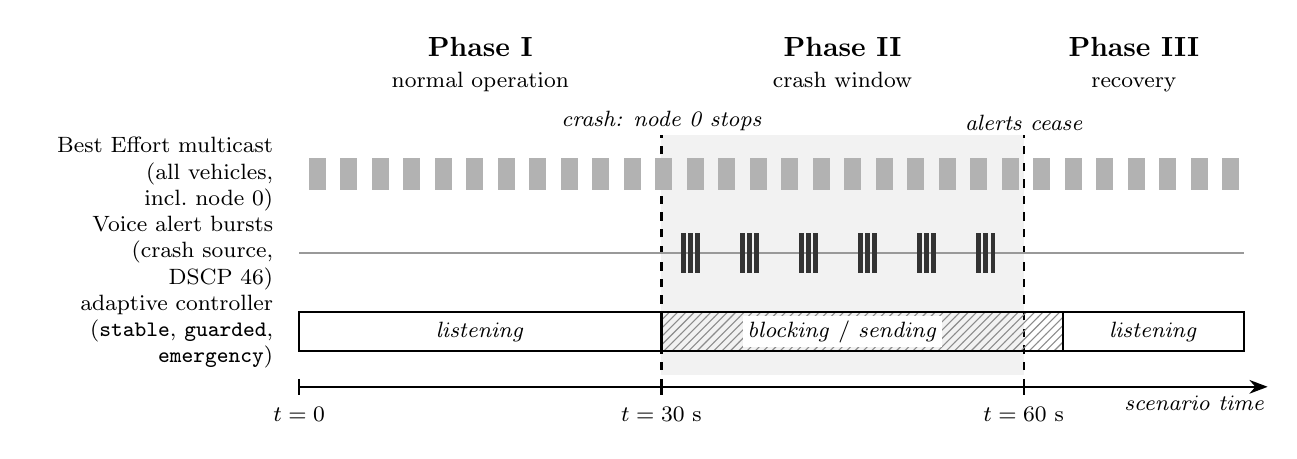
\begin{tikzpicture}[
  font=\small,
  >=Stealth,
  thick,
  lab/.style={font=\footnotesize\itshape, align=center, inner sep=1pt},
  rowlab/.style={font=\footnotesize, align=right, anchor=east, text width=3.0cm},
]
  % x positions: t=0 at 0, crash at \tc (30 s), window end at \te (60 s), horizon arrow beyond \tz
  \def\tc{4.6}
  \def\te{9.2}
  \def\tz{12}

  % ===== Phase headers =====
  \foreach \x/\p/\d in {{\tc/2}/{Phase I}/{normal operation}, {(\tc+\te)/2}/{Phase II}/{crash window}, {(\te+\tz)/2}/{Phase III}/{recovery}}{
    \node[font=\normalsize\bfseries, anchor=base] at ({\x},4.05) {\p};
    \node[font=\footnotesize, anchor=base] at ({\x},3.65) {\d};
  }

  % shaded crash window
  \fill[black!5] (\tc,0.0) rectangle (\te,3.05);
  \draw[thick, dashed] (\tc,-0.15) -- (\tc,3.05);
  \draw[thick, dashed] (\te,-0.15) -- (\te,3.05);

  % ===== Row 1: Best Effort background traffic (all vehicles) =====
  \node[rowlab] at (-0.2,2.55) {Best Effort multicast\\(all vehicles, incl.\ node~0)};
  \foreach \x in {0.12,0.52,...,11.8}{
    \fill[black!30] (\x,2.35) rectangle ++(0.22,0.4);
  }

  % ===== Row 2: Voice alert bursts (crash source) =====
  \node[rowlab] at (-0.2,1.55) {Voice alert bursts\\(crash source, DSCP~46)};
  \draw[black!40] (0,1.55) -- (\tz,1.55);
  \foreach \x in {4.85,5.6,...,8.9}{
    \foreach \k in {0,0.09,0.18}{
      \fill[black!80] (\x+\k,1.3) rectangle ++(0.06,0.5);
    }
  }

  % ===== Row 3: adaptive controller mode =====
  \node[rowlab] at (-0.2,0.55) {adaptive controller\\(\texttt{stable}, \texttt{guarded}, \texttt{emergency})};
  \draw[thick, fill=white] (0,0.3) rectangle (\tc,0.8);
  \node[font=\footnotesize] at (\tc/2,0.55) {\emph{listening}};
  \draw[thick, pattern=north east lines, pattern color=black!45] (\tc,0.3) rectangle (\te+0.5,0.8);
  \node[font=\footnotesize, fill=white, inner sep=1.5pt] at ({(\tc+\te)/2},0.55) {\emph{blocking} / \emph{sending}};
  \draw[thick, fill=white] (\te+0.5,0.3) rectangle (\tz,0.8);
  \node[font=\footnotesize] at ({(\te+0.5+\tz)/2},0.55) {\emph{listening}};

  % ===== Time axis =====
  \draw[->] (0,-0.15) -- (\tz+0.3,-0.15) node[lab, anchor=north east, yshift=-2pt] {scenario time};
  \foreach \x/\t in {0/{$t=0$}, \tc/{$t=30$~s}, \te/{$t=60$~s}}{
    \draw (\x,-0.05) -- (\x,-0.25);
    \node[font=\footnotesize, anchor=north] at (\x,-0.28) {\t};
  }

  % ===== Event annotations =====
  \node[lab, anchor=south] at (\tc,3.05) {crash: node~0 stops};
  \node[lab, anchor=south] at (\te,3.05) {alerts cease};
\end{tikzpicture}
\end{document}
